%================================================================================
%       Safety Critical Systems Club - Data Safety Initiative Working Group
%================================================================================
%                       DDDD    SSSS  IIIII  W   W   GGGG
%                       D   D  S        I    W   W  G   
%                       D   D   SSS     I    W W W  G  GG
%                       D   D      S    I    WW WW  G   G
%                       DDDD   SSSS   IIIII  W   W   GGG
%================================================================================
%               Data Safety Guidance Document - LaTeX Source File
%================================================================================
%
% Description:
%   Appendix regarding tool issues and seletion
%================================================================================
\section{Data Cygnology (Informative)}\index{Data Cygnology}\label{bkm:cygnology}
%
\dsiwgSectionQuote{Here be dragons}{Anon}

\subsection{Introduction}
The term “Black Swan” is used to describe an unpredictable event that is beyond what is normally expected of a situation and has potentially severe consequences.
Black Swan events were originally discussed in a financial context by Nassim Taleb in his 2004 book
\dsiwgTextIT{“Fooled By Randomness”} \cite{citation:cyg:RoleOfChance}
and further expanded to cover other topics in
\dsiwgTextIT{“The Black Swan: The Impact of the Highly Improbable”}
\cite{citation:cyg:BlackSwan}.
The term quickly became accepted, and Black Swan events are characterized by their extreme rarity, severe impact, and the widespread insistence they were obvious in hindsight. Taleb gave examples such as the rise of the Internet, the personal computer and financial crashes as “Black Swan” events, but the term can equally be applied to unexpected safety-related events such as the Boeing 737 MAX crashes of 2018 / 2019 \cite{citation:cyg:737Max}.

While Black Swans are events that are only obvious in hindsight, other types of event may be extremely rare and have severe impact but are predictable beforehand, for example pandemics.
Another example comes from the sun:  a Coronal Mass Ejection (CME) of such severity can be produced that it causes widespread life-threatening electromagnetic interference on Earth.
This type of event can be predicted to occur to some extent, and has happened before, for example the “Carrington Event” of 1859 \cite{citation:cyg:carrington}.
These rare events which have rapid escalation, but are somewhat predictable are termed “Dragon King” events.

There are several more event types noted in the literature.
The practice of studying these types of high-impact but rare variants has been termed “Cygnology”,
a term that appears in work by Ale, Hartford and Slater in their “Dragons,
black swans and decisions” paper of 2020 \cite{citation:cyg:dragons}.

While Cygnology can be applied to safety in general,
it can also be applied to data safety and recent research has identified four important
categorisations of data-related risks:
\begin{itemize}
\item Black Swan Data
\item Dragon King Data
\item Perfect Storm Data
\item Pudding Lane Data
\end{itemize}

These types of data are discussed in more detail in the following sections along with recommended strategies for managing their associated risks.

\subsection{Black Swan Data}\index{Data Cygnology!Black Swan Data}
\dsiwgTextBF{Definition:} Data that is totally unexpected by those receiving it (i.e. ‘out of the blue’) and has huge (detrimental) impact, but in retrospect should have been anticipated.

\begin{wrapfigure}{R}{0.25\textwidth}
  
\includegraphics{images/cygSwan}
\end{wrapfigure}

In 2013, a C-130 Hercules aircraft landed at Bar Yehuda airport near the Dead Sea, a saltwater lake sitting astride Israel and Jordan. The Dead Sea is the lowest place on Earth and the airfield lies -1,210 feet below sea level.

The aircraft's navigation system became unresponsive and the constellation of \gls{gps} satellites above, mysteriously winked out of existence. As it turned out, the plane's navigation electronics were not designed to operate at altitudes less than 400 feet below mean sea level. In a sense, the plane thought it was underwater.

This is an example of what is termed a “Black Swan Data” event; the stream of altitude data going to the navigation systems surprisingly turned significantly negative and could have had a catastrophic result; a situation not considered possible. Yet, with hindsight, and knowledge of earth’s geography, we can rationalise this and question why the assumption of positive altitude data was ever thought to be true in the first place.

\subsubsection{Managing Black Swan Data Risks}
The following strategies are recommended for managing Black Swan Data Risks:
\begin{itemize}
\item Be aware of changes of usage, environmental conditions or failures that may produce data
that is not expected.
The Ariane 501 launch disaster may be thought of in these terms,
as the horizontal bias values that caused the exception leading to the complete loss of mission
were not anticipated;
\item Continually test the established thinking; challenge the oft quoted
“that’s just how we do things around here”;
\item What assumptions have been made about the data?
Are these really valid and do they continue to be valid in a changing and dynamic world?
\item What happens if different inputs (e.g. new sensors or \gls{information} flows)
are added to your system?
\item Think outside the box;
it is the most wild and implausible (compared to current perceptions)
ideas that will trip a Black Swan Data event --
what could possibly be ‘bad data’ and how might it be handled?
\end{itemize}

\subsection{Dragon King Data}\index{Data Cygnology!Dragon King Data}
\dsiwgTextBF{Definition:} Data whose effect might have been foreseen, but leads to an unexpected and explosive escalation
with major impact (‘things get rapidly out of control’).

\begin{wrapfigure}{R}{0.25\textwidth}
  
\includegraphics{images/cygDragon}
\end{wrapfigure}

In risk management a Dragon King is defined as an event that is both extremely large in size
or impact (a "king") and born of unique origins (a "dragon") relative to other events in the system.

Dragon King events are generated by, or correspond to, mechanisms such as positive feedback,
tipping points, bifurcations, and phase transitions that tend to occur in non-linear and complex
systems, and serve to amplify events to extreme levels.
In the data domain, “Dragon King Data” represents incorrect or missing data whose consequences
unexpectedly escalate into an unpredicted and often catastrophic system event.

An example might be the loss of data relating to Covid-19 test results in the UK due to a row limit
in Microsoft Excel.
This led to Public Health England losing 15,841 positive test results, which in turn,
meant that 50,000 potentially infectious people were missed by contact tracers and not told to
self-isolate.
Because of the exponential way that viruses spread,
this may have led to many more infections and deaths.

Another, older, example is the infamous comment given by the weather forecaster Michael Fish
about the Great Storm of 1987:

\begin{quote}
"Earlier on today, apparently, a woman rang the BBC and said she heard there was a hurricane on the way. Well, if you're watching, don't worry, there isn't!"
\end{quote}

These few words may well have led to precautions not being taken across the whole of Southern
England, affecting millions of people.
In fact, the storm was the worst to hit South East England for three centuries,
causing record damage and killing 19 people.

\subsubsection{Managing Dragon King Data Risks}
The following strategies are recommended for managing Dragon King Data Risks:
\begin{itemize}
\item Identify all the receiving systems or users of the data:
what are the consequences of errors or losses in the data to those receiving it?
\item Analyse the effects of data impact: are any effects subject to non-linear effects?
Try to establish the consequence chains and knock-on effects;
\item Do any of the data potentially impact systems that have large fan-out or spread?
\item Create models (or even Digital Twins) of the system in a way that different combinations
of data can be tested and simulated to reveal extreme non-linear behaviours.
\end{itemize}

\subsection{Perfect Storm Data}\index{Data Cygnology!Perfect Storm Data}
\dsiwgTextBF{Definition:} Combinations, sets or occurrences of data (or absences of data) that would never have been thought possible to occur together, and when they do have a large and undesirable impact.

\begin{wrapfigure}{R}{0.25\textwidth}
  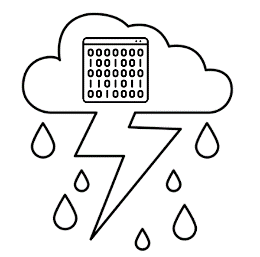
\includegraphics{images/cygStorm}
\end{wrapfigure}

A Perfect Storm in the risk world is when everything bad happens at the same time,
and it was not anticipated that this could happen.
These risks get their name from “The Perfect Storm”,
both a 2000 American biographical disaster drama film \cite{citation:perfectstorm:website}
and a 1997 non-fiction book by Sebastian Junger \cite{citation:perfectstorm:book}.
In the data world, a Perfect Storm is when the data that the system relies upon are all wrong
(or missing) at the same time, and can be layers deep – much akin to Reason’s Swiss cheese model.
A classic example might be to try and restore deleted data from a backup system,
only to find that the backups had not been working properly due to a configuration problem.
Perfect Storm Data is therefore when multiple data faults or losses conspire to create a
situation that has disproportionately catastrophic outcomes.

Another example is from the world of security;
on 10th Dec 2021, a new critical zero-day vulnerability was detected that affected
Apache Log4j 2 Java library.
It adversely impacted the digital domain and security systems worldwide.
The vulnerability, when exploited, permitted remote code execution on the vulnerable server
with system-level privileges.
The exploit was a combination of both the Java code that contains different logging functions
and the settings of a configuration file.

Another example is the China Airlines A333 at Taipei on 14th June 2020  when all primary computers,
reversers and auto brakes failed on touchdown.
During landing, flight controls reconfigured from ‘normal law’ to ‘direct law’ after all three
\glspl{fcpc} became inoperative.
While all aircraft primary control surfaces were still controllable,
the deceleration devices including ground spoilers, thrust reversers, and autobrake were lost;
the deceleration of the aircraft had to be performed by manual braking by the pilots.

\subsubsection{Managing Perfect Storm Data Risks}
The following strategies are recommended for managing Perfect Storm Data Risks:
\begin{itemize}
\item Analyse combinations of data that are important: how might one \gls{dataset} being wrong influence another?
\item Look at dependencies in the data: are seemingly different \glspl{dataset} all derived from a common source?
\item Examine as many levels of the system to establish commonalities and dependencies;
\item Even if no commonalities are found,
consider the unlikely cases of independent data being wrong together,
and follow through their consequences.
\end{itemize}

\subsection{Pudding Lane Data}\index{Data Cygnology!Pudding Lane Data}
\dsiwgTextBF{Definition:} Data that is unknowingly and unexpectedly critical to the whole operation and if missing or incorrect in some way, has a dramatic and negative impact. After the event it may be obvious that it was critical.

\begin{wrapfigure}{R}{0.25\textwidth}
  
\includegraphics{images/cygPudding}
\end{wrapfigure}
\begin{quote}
“Lord! what sad sight it was by moone-light to see, the whole City almost on fire,
that you might see it plain at Woolwich, as if you were by it”.
\end{quote}

These words from Samuel Pepys diary in 1666, give a personal account of the Fire of London that
destroyed 13,200 houses, 87 parish churches, The Royal Exchange, Guildhall and St. Paul’s Cathedral,
all from a single fire thought to have started in a humble baker’s shop in Pudding Lane.

In the same way, unexpectedly \gls{critical data} can also act as a catalyst to catastrophic outcomes
if the dependencies are not identified and adequately mitigated.
Often this data is part of an existing system and may be long forgotten
(e.g. a system configuration parameter).
It may also be a hard-wired parameter in legacy source code that code maintainers change because
they do not understand its original purpose.

In 2015, an Airbus A400M Atlas cargo plane on a test flight crashed at La Rinconada, Spain,
less than 5 kilometres from Seville Airport, killing 4 of the 6 crew.
Several reports suggested that as many as three of the aircraft's four engines failed during
the A400M's departure from Seville.

The suspected cause of the failure was that the torque calibration parameter data had been
accidentally wiped on three engines as the engine software was being installed,
which would prevent the engine control software from operating properly.
In this case, the seemingly innocuous calibration data had a critical role to play in the
safety of the entire platform and so the term “Pudding Lane Data” is coined to encompass
this form of data.

\subsubsection{Managing Pudding Lane Data Risks}
The following strategies are recommended for managing Pudding Lane Data Risks:
\begin{itemize}
\item Understand and know all the data.
The high-profile data streams will of course be first and foremost, but is there an inventory of
all the data that the system depends upon and are the implications if there is loss of their \glspl{data property} understood? 
\item Configuration and tailoring data may seem static and uninteresting but what are the
dependencies on this data?
If loss of properties of this data can have catastrophic outcomes,
then what processes and mitigations will be put in place to assure those properties are maintained?
\item Consider the reporting and monitoring data: if this is incorrect will poor decisions be taken?
\end{itemize}

\subsection{Conclusions}
Looking at Data Risks through Cygnology can help to tease out some unlikely but severe failures of systems involving data. It is possible that sometimes these risks are already considered in system \gls{hazop} sessions but discounted as too unlikely to happen. The Data Cygnology approach is recommended as a useful and visual ‘Tool in the Box’ when trying to identify extreme data-related risks of systems.
Due to their serious impact arguably they should still be included, assessed and managed alongside more ‘normal’ risks.

\subsection{Summary Table}\index{Data Cygnology!Summary}
\begin{longtable}{|C{\dsiwgColumnWidth{0.2}}|L{\dsiwgColumnWidth{0.4}}|C{\dsiwgColumnWidth{0.2}}|}
  \caption{Summary of cygnology types}
  \label{tab:cygnologytypes}
  \\\hline
%  \TableHeadColour{} & \multicolumn{3}{c|}{\TableHeadColourCX{Likelihood}}\\\cline{2-4}
  \TableHeadColourCX{Type} & \TableHeadColourCX{Brief Explanation} & \TableHeadColourCX{Icon}\\\hline
  \endfirsthead
  \caption[]{Summary of cygnology types (continued)}
  \\\hline
%  \TableHeadColour{} & \multicolumn{3}{c|}{\TableHeadColourCX{Likelihood}}\\\cline{2-4}
  \TableHeadColourCX{Type} & \TableHeadColourCX{Brief Explanation} & \TableHeadColourCX{Icon}\\\hline
  \endhead
  \multicolumn{3}{r}{\sl Continued on next page}
  \endfoot
  \endlastfoot
  Black Swan Data &
  Data that is totally unexpected by those receiving it (i.e. ‘out of the blue’)
  and has huge (detrimental) impact, but in retrospect should have been anticipated. &
  
\includegraphics[scale=0.55]{images/cygSwan}
  \\\hline 
  %
  Dragon King Data &
  Data whose effect might have been foreseen,
  but leads to an unexpected and explosive escalation with major impact
  (‘things get rapidly out of control’). &
  
\includegraphics[scale=0.55]{images/cygDragon}
  \\\hline
  %
  Perfect Storm Data &
  Combinations, sets or occurrences of data (or absences of data)
  that would never have been thought possible to occur together,
  and when they do have a large and undesirable impact. &
  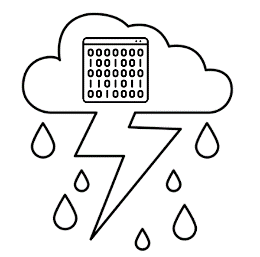
\includegraphics[scale=0.55]{images/cygStorm}
  \\\hline
  %
  Pudding Lane Data &
  Data that is unknowingly and unexpectedly critical to the whole operation and if missing
  or incorrect in some way, has a dramatic and negative impact.
  After the event it may be obvious that it was critical. &
  
\includegraphics[scale=0.55]{images/cygPudding}
  \\\hline
\end{longtable}

